\newpage
%——————————————————————设置开始计数———————————————————
\setcounter{page}{1}
\cfoot{\thepage}

\section{绪论}
\subsection{背景与意义}

近十年来,中国乃至全世界的老龄化愈发严重,促进了人们对行动不便的人士伤病护理的重视程度的提高。与此同时,机电设备的发展也到达了新的高度,科技人员将机电技术应用在一些日常生活用品,如本文的建模对象,也即手动轮椅,从而到达智能化,机电一体化的在生活护理方面的应用。

患有认知/运动/感觉障碍的人,可以依靠电动轮椅来满足他们的行动需求。 由于一些残疾人无法使用传统的操纵杆导航他们的轮椅,他们使用替代控制系统,如手动操纵杆,手指操纵杆(图\ref{fig:smart_wheel_chairs}所示)。 在许多情况下,电动轮椅使用者在日常操纵任务方面存在困难,并且将受益于自动导航系统。

%%%%%%%%%%%%%%%%%
\begin{figure*}[!h]
	\centering
	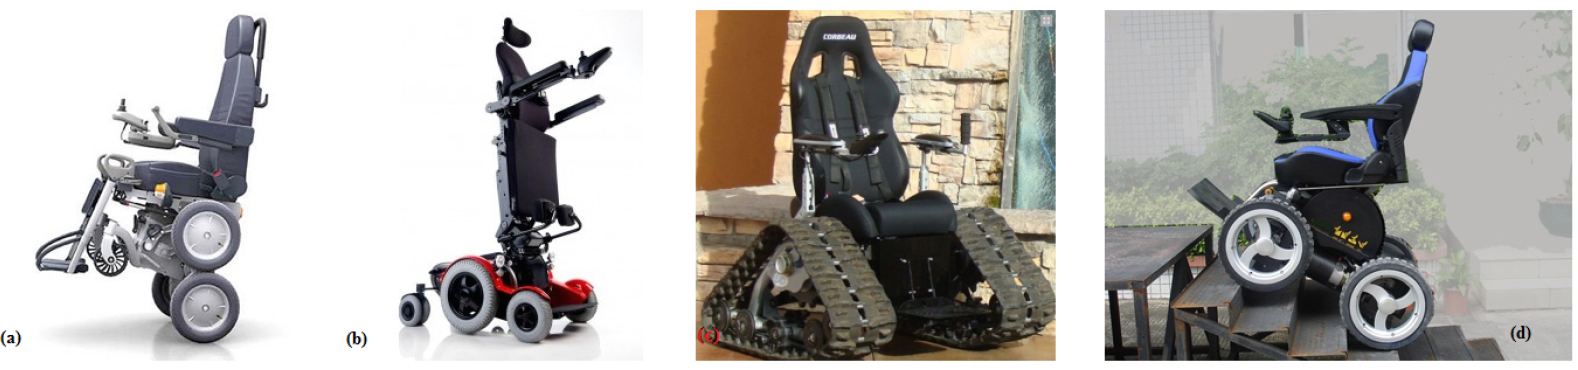
\includegraphics[width=1\textwidth]{fig/smart_wheel_chairs.png}
	\caption{近几年电动轮椅案例。}\label{fig:smart_wheel_chairs}
\end{figure*}
%%%%%%%%%%%%%%%%%

因此本文建模对象为电动轮椅中的机械与电驱动部分,如图\ref{fig:PW_rendering}所示。
首先,我们以两轮机器人系统理论应用与手动轮椅主体部分的分析,在此基础上,结合包括了电源,电机与驱动轮的便携式机电驱动模块(MDM, mechatronic drive modules) 。该模块可以在必要时与大规模的手动轮椅系统耦合,以提高推进效率,从而给整体系统带来了很好的优势,因为模块的重量被施加在模块本身上,从而防止了结构的变形。考虑到复杂程度和所学知识,我们进行合理假设与简化模型,取整体系统的机械主体和附加几点模块,进行运动学仿真与键合图建模。

%%%%%%%%%%%%%%%%%
\begin{figure*}[!h]
	\centering
	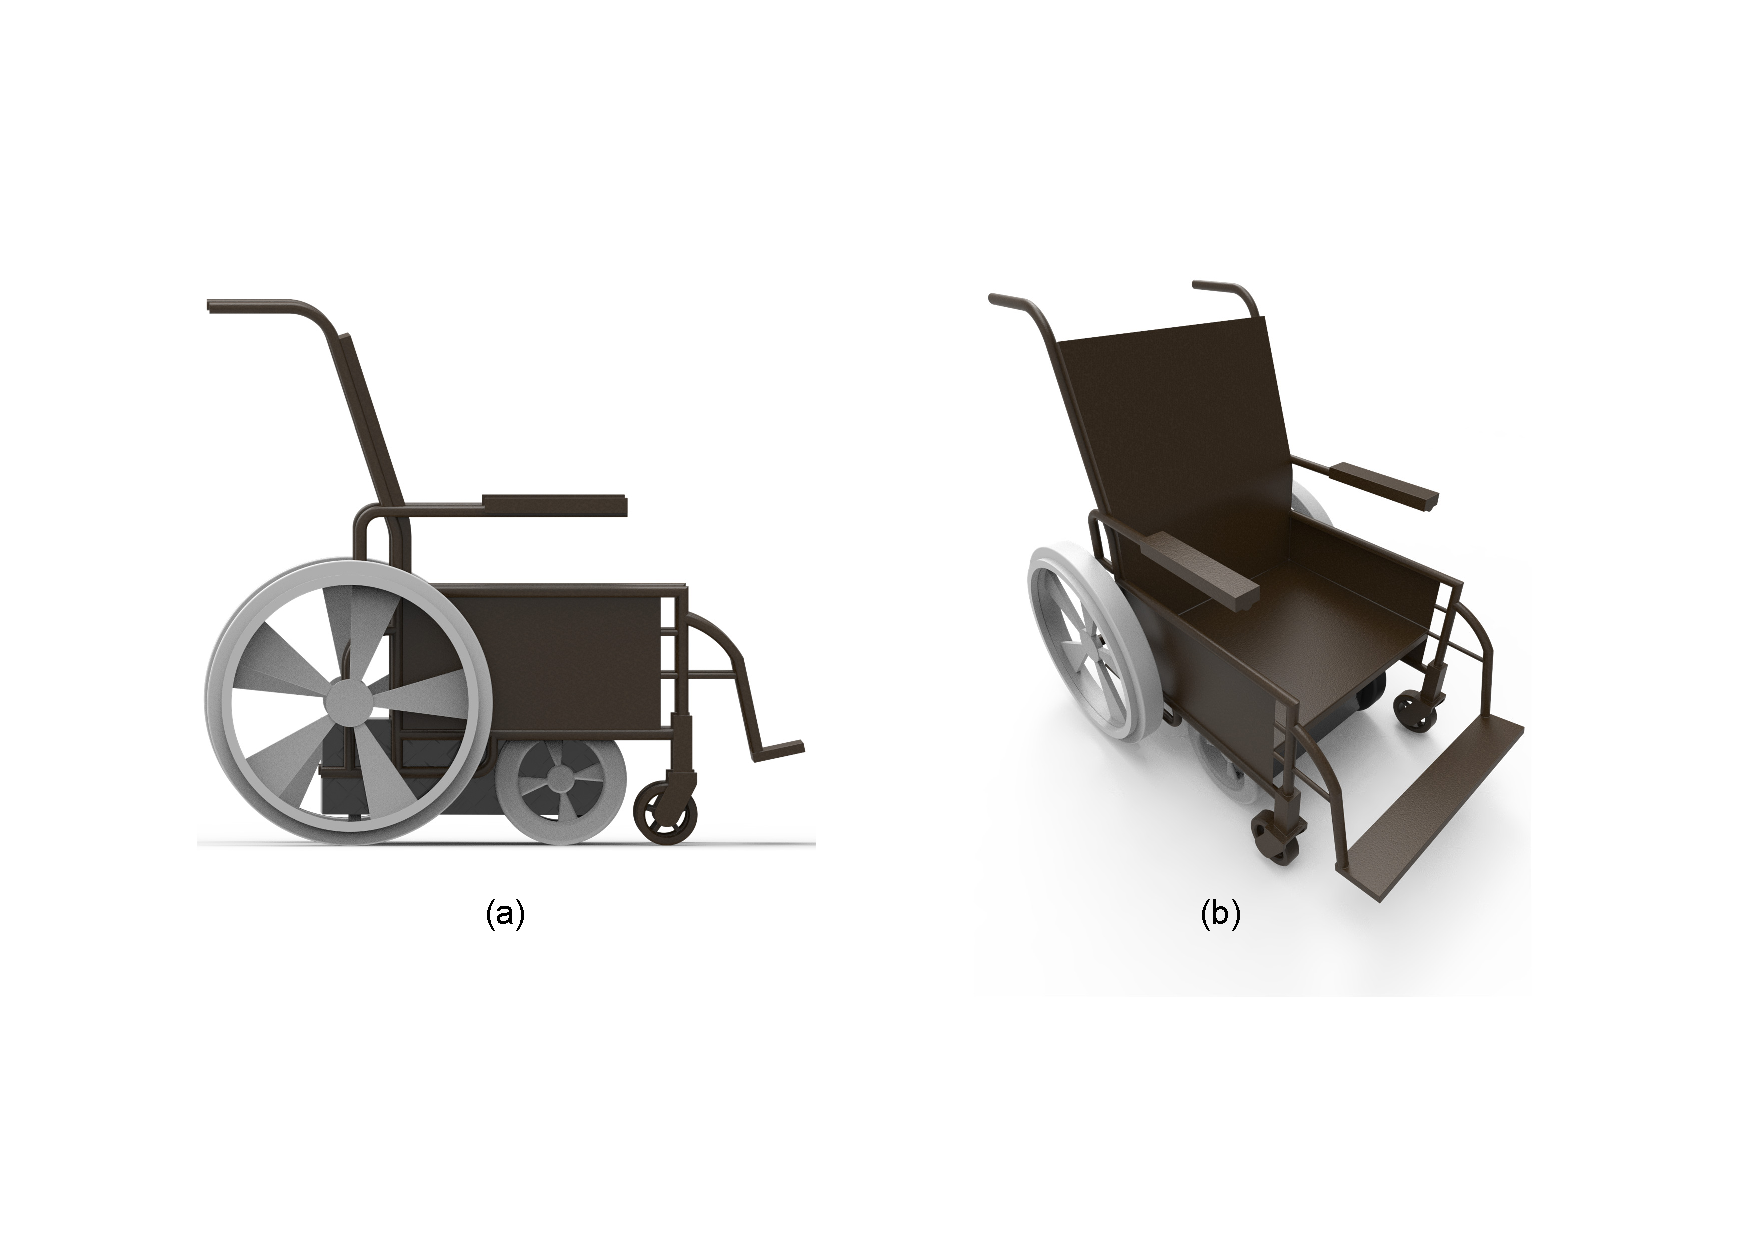
\includegraphics[width=1\textwidth]{fig/PW_rendering.pdf}
	\caption{选取电动轮椅示意。(a) 和 (b) 分别表示建模对象的侧视图和立体视图。}\label{fig:PW_rendering}
\end{figure*}
%%%%%%%%%%%%%%%%%

\subsection{本报告章节安排}

本报告从建模对象出发,从手推轮椅主体和机电驱动模块两部分出发进行分析建模,然后两部分结合进行系统整体分析总结,最后给出参考文献,报告主体内容包括以下几个部分:

第二章是对建模对象进行描述和问题提取,并给出相关模型合理假设以及参数标记;

第三章是对手推轮椅主体运动学分析和键合图建模;

第四章是对机电驱动模块的分析与键合图建模;

第五章是整体键合图的给出,并给出总结和分析;

最后部分为本文参考文献。